% Ornith-1.5-9B distillation paper.
% Compile from the paper/ directory with: tectonic main.tex
% Tables are generated from measured artifacts:  uv run python scripts/make_paper_tables.py

\documentclass[11pt]{article}

\usepackage[utf8]{inputenc}
\usepackage[T1]{fontenc}
\usepackage[margin=1in]{geometry}
\usepackage[hidelinks]{hyperref}
\usepackage{url}
\usepackage{booktabs}
\usepackage{amsfonts}
\usepackage{amsmath}
\usepackage{amssymb}
\usepackage{microtype}
\usepackage{graphicx}
\usepackage{xcolor}
\usepackage{multirow}
\usepackage{array}
\usepackage{enumitem}
\usepackage[numbers]{natbib}
\newcolumntype{L}[1]{>{\raggedright\arraybackslash}p{#1}}
\emergencystretch=2em

\newcommand{\HALT}{\textsc{HALT}}
\newcommand{\Student}{Ornith-1.5-9B}
\newcommand{\oQ}{\texttt{oQ4}}
\newcommand{\RepoURL}{\url{https://github.com/adityak74/ornith-1.5-9b-distil}}
\newcommand{\PRURL}{\url{https://github.com/ml-explore/mlx-lm/pull/1870}}
% Headline numbers for the abstract; Tables~\ref{tab:forcing} and \ref{tab:soft} have the full set.
\newcommand{\Forcinghighlight}{+10.4 points of HumanEval on the stock quantized build and +7.3 on the distilled one}
\newcommand{\Softhighlight}{+18.9 points on the stock build (108 to 139 of 164) and +10.4 on the distilled one at a 2{,}048-token budget, with no item that was correct becoming wrong}
\newcommand{\Generalhighlight}{the 3-bit, 4-bit, 8-bit and full-precision builds and the 35B teacher all gain, by two thirds to four fifths of whatever truncated, with one regression in 735 previously-correct items}

\title{\HALT{}: Quantized Reasoning Models Don't Stop,\\
and a Harness-Applied Limit on Thinking Repairs Them}

\author{%
  Aditya Karnam Gururaj Rao\\
  \texttt{adityakarnam.grao@gmail.com}\\[0.6em]
  Arjun Jaggi\\
  \texttt{arjunjaggi@gmail.com}\\
}
\date{}

\begin{document}

\maketitle

\begin{abstract}
Quantizing \Student{}, a 9B hybrid-attention reasoning model, to 4.7 bits costs
4.6 points of MMLU and 3.7 of HumanEval against its bf16 parent.  We set out to
recover that loss by distillation and, over three weeks on a single 64\,GB
Apple M4 Pro, tried twelve things.  The first worked: two-teacher sequence-level
distillation with rejection sampling on verified traces, trained in bf16 and
quantized last, gives a model at identical size and bit width that scores
+5.5 MMLU and +3.0 HumanEval over the quantized baseline, beats the
1.8$\times$ larger 8-bit build on both, and matches its own 35B teacher on
MMLU---while generating 15--33\% fewer tokens.  Nine training-side variants did
not: data mixture, volume, length distribution, training objective, filter,
adapter capacity, on-policy prompt selection, self-distillation of the
model's own terminated traces, and preference training against its own
unterminated ones all failed to improve on it, and a randomised control showed
that a second training pass from the best checkpoint costs 1--4 points
regardless of what it trains on.  Diagnosing \emph{why} the
first run worked turned out to be the useful result: most of what quantization
costs this model is not reasoning ability but the ability to \emph{stop}.  The
4-bit build fails to reach an answer on 24\% of HumanEval problems its parent
finishes, 22 of the 28 problems distillation recovered were budget exhaustions,
and the effect reproduces as wall clock on a harness with no truncation penalty.
The two repairs that worked followed from that diagnosis and needed no training
at all.  \HALT{}, a Harness-Applied Limit on Thinking, in its hard form closes
the reasoning block at the decode budget and lets the model answer, recovering
\Forcinghighlight{} on the same quantized weights.  In its soft form it adds a
bias to the \texttt{</think>} logit that grows with position, so the model
chooses where to stop but stopping gets steadily cheaper: this recovers
\Softhighlight{}, beats the hard form, and at 2{,}048 tokens outscores the
full-precision parent at 4{,}096.  The ramp is not a quantization repair:
\Generalhighlight{}.  Every build over-thinks at a fixed budget; quantization
raises how often, so the quantized builds have the most to recover.  We
conclude that termination is a decoding-time property before it is a weights
property, that any benchmark of a reasoning model that does not report its
truncation rate is partly reporting its own token budget, and we
release the pipeline, every checkpoint, per-item evaluation records and a
53-section decision log.  Along the way we contribute a chunkwise-parallel
training path for gated DeltaNet layers in MLX (24$\times$ memory, 135$\times$
speed at 4{,}096 tokens), now upstream.
\end{abstract}

\section{Introduction}

Post-training quantization is how a reasoning model reaches consumer hardware,
and its cost is customarily reported as a few points of benchmark accuracy.
This paper asks what those points \emph{are}.  It began as a distillation
project---recover the quantization loss by teaching the 4-bit model from larger
ones---and it succeeded on the first attempt.  It then spent seven further runs
failing to improve on that success, each moving one variable with a prediction
recorded before measurement, until the accumulated negative results and the
per-item evaluation records forced a different question: not \emph{what did
the successful run teach the model}, but \emph{what was broken that it fixed}.

The answer is that the quantized model does not stop.  On a strict harness at a
4{,}096-token budget, stock \oQ{} \Student{} never reaches an answer on 39 of
164 HumanEval problems; its bf16 parent truncates on 15.  The distilled model
truncates on 19, and 22 of the 28 problems it gains over stock are ones where
stock ran out of budget mid-reasoning.  Along the quantization ladder, the
3-bit build takes 2.2$\times$ as long as the 4-bit build to answer the same
questions while scoring 11 points lower, despite having fewer bits to
multiply.  The same bf16 weights score 82.3\% or 88.4\% on HumanEval depending
only on whether the budget is 2{,}048 or 4{,}096 tokens.

Once the failure is named, the cheapest repair is obvious: stop the model for
it.  We call the result \HALT{}, a Harness-Applied Limit on Thinking, and it
comes in two forms.  The hard form is the closing half of budget forcing
\citep{muennighoff2025s1}, applied as a two-phase decoder that closes the
reasoning block when the budget is nearly spent and lets the model commit.  The
soft form is a single logits processor: a bias on the \texttt{</think>} token
that grows linearly with position once reasoning has run past a threshold, so
the model still chooses where to stop, but stopping gets cheaper the longer it
goes on.  Neither is a training run.  The soft form recovers 31 of 164
HumanEval problems on the stock 4-bit build with no regressions, and it turns
out not to be about quantization at all: the same ramp lifts the bf16 parent
by 17 and the 35B teacher by 8, and across six builds from 3 bits to full
precision the gain is a fixed fraction of what truncated.  Two training-side
attempts to move the behaviour into the weights both failed, which is
consistent with it being a property of greedy decoding under a finite budget
rather than of anything the weights encode.

\paragraph{Contributions.}
\begin{enumerate}[leftmargin=1.5em]
  \item A training-side repair (\S\ref{sec:method}--\ref{sec:main}): two-teacher
    sequence-level distillation with rejection sampling, +5.5 MMLU and +3.0
    HumanEval at identical size and bit width.
  \item A diagnosis (\S\ref{sec:mechanism}): quantization damages termination
    more than reasoning, evidenced six ways, including in the 35B teacher.
  \item A decoding-side repair (\S\ref{sec:forcing}): \HALT{}, a harness-applied
    limit on thinking, in a hard (two-phase) and a soft (logit ramp) form, on
    the same weights, with the finding that stopping \emph{earlier} than the
    model would stop itself improves accuracy, that the soft form does so with
    one regression in 735 items across six builds, and that the gain tracks
    the truncation count from 3 bits to full precision and from 9B to 35B.
  \item Ten controlled negative results (\S\ref{sec:negative}), including a
    randomised control showing that continued training from the best checkpoint
    is itself harmful, evidence that the teacher cannot supply the one
    behaviour the student lacks, and two failed attempts to train the
    \HALT{} behaviour into the weights.
  \item An engineering result (\S\ref{sec:engineering}): a differentiable
    chunkwise training path for gated DeltaNet in MLX, contributed upstream.
\end{enumerate}

\section{Setup}
\label{sec:setup}

\paragraph{Student.}
\Student{} is a 32-layer hybrid-attention reasoning model with gated DeltaNet
(GDN) linear-attention layers \citep{yang2024gated}, a 248{,}044-token
vocabulary and a thinking-mode chat template that opens a \texttt{<think>}
block before every answer.  The deployed quantization, \oQ{}, is 4-bit affine
at group size 64 with 120 modules (predominantly linear-attention projections)
promoted to 5, 6 or 8 bits, averaging 4.721 bits per weight.  The promotion map
is recoverable from the checkpoint's configuration and we replay it exactly, so
every quantized comparison in this paper is like-for-like rather than ``our
4-bit against theirs''.

\paragraph{Teachers.}
Two 35B-A3B mixture-of-experts models at 4 bits, routed by measured strength
rather than reputation (Table~\ref{tab:teachers}).  Qwen3.6-35B-A3B is 6.3
points stronger on MMLU and teaches knowledge and truthfulness; Ornith-1.5-35B
ties it on HumanEval while sampling 4.6$\times$ faster and teaches code.  All
three models share an index-identical vocabulary (verified: vocabulary and
merges equal; Qwen's pre-tokenizer regex differs, affecting text encoding but
not token identity), which is what makes logit-level distillation
(\S\ref{sec:v5}) possible at all.

\begin{table}[t]
\centering
\caption{Teachers, measured under the same protocol as the student.}
\label{tab:teachers}
\begin{tabular}{lrrrr}
\toprule
Teacher & MMLU & TruthfulQA & HumanEval & Sampling speed \\
\midrule
Qwen3.6-35B-A3B, 4-bit & \textbf{89.3} & \textbf{89.2} & 93.3 & 1.0$\times$ \\
Ornith-1.5-35B-A3B, 4-bit & 83.0 & 86.4 & 93.3 & \textbf{4.6}$\times$ \\
\bottomrule
\end{tabular}
\end{table}

\paragraph{Benchmarks and protocol.}
MMLU \citep{hendrycks2021mmlu} on a fixed seeded 1{,}000-question sample of
14{,}042; TruthfulQA MC1 \citep{lin2022truthfulqa}, all 817; HumanEval
\citep{chen2021humaneval}, all 164.  Thinking enabled, greedy decoding.  Two
harnesses were used.  The oMLX server is the deployment target and the source
of every headline number.  Our own harness (\texttt{odistil eval}) records
per-item truncation, token counts and wall clock, and is what the mechanism
analysis rests on.  The two disagree by up to 15 points on the \emph{stock}
model's HumanEval, because oMLX recovers an answer from output ours scores as
unfinished; they agree on every direction, and no table mixes them.

\paragraph{Evaluation hygiene.}
TruthfulQA lists the correct choice first in all 817 items.  Presented in
dataset order, every gold answer is ``A'', and a model that always answers A
scores 100\%; an early version of our harness did exactly this and reported a
metric that was measuring position bias.  We shuffle choices under a per-item
seed.  Model-generated code runs only in a subprocess with a temporary working
directory and a hard timeout.  Training data is decontaminated against all
three evaluation sets by 13-gram overlap.

\paragraph{Hardware.}
One Apple M4 Pro with 64\,GB of unified memory.  A full fine-tune of a 9B does
not fit ($\approx$18\,GB of weights plus $\approx$72\,GB of fp32 AdamW state);
LoRA \citep{hu2022lora} over the bf16 base does.  Only one model is resident at
a time, which shapes every stage of the pipeline.

\section{Method: the run that worked}
\label{sec:method}

\paragraph{Sequence-level distillation with rejection sampling.}
Following \citet{kim2016sequence}, the student learns from teacher-generated
sequences rather than teacher logits.  For each prompt in a pool drawn from
MMLU auxiliary-train, ARC, OpenBookQA, TriviaQA, SciQ and MBPP, the owning
teacher generates one reasoning trace with thinking enabled.  The trace is
kept only if it verifies: final letter matches gold (multiple choice),
normalised answer matches a gold alias (open QA), or the extracted program
passes the dataset's own tests (code).  Qwen scores 89.3\% on MMLU, so roughly
one unfiltered knowledge trace in nine would be a confidently argued wrong
answer.  Traces exceeding the training length cap are dropped rather than
truncated: a truncated target teaches the model to stop mid-answer, which is
the opposite of what \S\ref{sec:mechanism} shows it needs.

\paragraph{Train in bf16, quantize last.}
LoRA at rank 32 over the top 16 of 32 layers ($\alpha=16$, dropout 0.05),
3{,}200 steps at batch size 1, learning rate $3\times10^{-5}$ with cosine decay
and 150 warmup steps, 1{,}024-token cap.  Adapters are fused into a bf16
checkpoint, which is then quantized with the replayed \oQ{} map, so the
quantizer starts from an improved checkpoint instead of compounding two lossy
steps.  QLoRA \citep{dettmers2023qlora} over the quantized base was measured and
rejected: 49.0\,GB peak against bf16's 47.3 and 26\,s per iteration against 10,
because dequantising every step costs more than the smaller weights save.

\paragraph{Mixture.}
40\% knowledge, 25\% truthfulness, 35\% code by sample count, sized from
whichever domain is most over-supplied so that scarcity in one domain never
discards verified data in another.  The run we call v1 trained on 1{,}639
samples with 33 held out.

\section{Main result}
\label{sec:main}

\begin{table}[t]
\centering
\caption{Main result. All rows measured on the oMLX server under the same protocol (MMLU: fixed 1{,}000-question sample; TruthfulQA: all 817; HumanEval: all 164; thinking on; greedy). Size is the on-disk checkpoint. The distilled model is quantized with the identical oQ4 map as the stock build.}
\label{tab:main}
\begin{tabular}{lrrrrr}
\toprule
Model & GB & MMLU & TruthfulQA & HumanEval & HumanEval s \\
\midrule
Ornith-1.5-9B oQ3 & 3.9 & 66.6 & 67.6 & 72.0 & 5,585 \\
Ornith-1.5-9B oQ4 (stock) & 4.9 & 78.0 & \textbf{80.7} & 87.8 & 4,171 \\
Ornith-1.5-9B oQ8 & 8.9 & 83.1 & 80.7 & 88.4 & 4,797 \\
Ornith-1.5-9B bf16 & 17 & 82.6 & 80.5 & \textbf{91.5} & 9,994 \\
\midrule
\textbf{distilled oQ4 (v1, ours)} & \textbf{4.9} & \textbf{83.5} & 79.0 & 90.8 & 2,786 \\
\midrule
Ornith-1.5-35B-A3B 4-bit (teacher) & 18 & 83.0 & 86.4 & 93.3 & 1,043 \\
Qwen3.6-35B-A3B 4-bit (teacher) & 19 & 89.3 & 89.2 & 93.3 & 4,804 \\
\bottomrule
\end{tabular}
\end{table}


Table~\ref{tab:main} gives the result.  Against the model it replaces, the
distilled \oQ{} build is \textbf{+5.5 MMLU and +3.0 HumanEval at identical size
and bit width}, and $-1.7$ TruthfulQA.  It beats the 1.8$\times$ larger 8-bit
build on both gains, edges the 3.5$\times$ larger bf16 parent on MMLU, and
matches its own 35B code teacher on MMLU.  It is also faster: $-33\%$ wall clock
on HumanEval and $-15\%$ on MMLU against stock---the same weights per token,
fewer tokens per answer.  The TruthfulQA regression is real and is analysed in
\S\ref{sec:truthfulqa}.

This was the first run.  Sections~\ref{sec:negative} describes the seven that
followed it and failed.  Section~\ref{sec:mechanism} explains why the first one
worked, which is what eventually pointed at the ninth.

\section{The mechanism: quantization breaks stopping}
\label{sec:mechanism}

\subsection{Truncation explains the gain}

On our harness at a 4{,}096-token HumanEval budget, with both models quantized
by the identical map (Table~\ref{tab:trunc}), the distilled model gained 28
problems over stock and lost 8.  \textbf{Twenty-two of the 28 gains were
problems on which the stock model ran out of budget mid-reasoning.}  The gain is
not mostly new capability; it is mostly finishing.  Truncation falls on every
benchmark at once: MMLU 24$\to$10, TruthfulQA 27$\to$20, HumanEval 39$\to$19.

\begin{table}[t]
\centering
\caption{Stock and distilled \oQ{} on our harness, HumanEval, 4{,}096-token budget.}
\label{tab:trunc}
\begin{tabular}{lrr}
\toprule
 & Stock \oQ{} & Distilled \oQ{} \\
\midrule
HumanEval & 72.0\% & \textbf{84.1\%} \\
Never reached an answer & \textbf{39 / 164 (24\%)} & \textbf{19 / 164 (12\%)} \\
Mean generation (tokens) & 1{,}721 & \textbf{1{,}414} \\
\bottomrule
\end{tabular}
\end{table}

\begin{figure}[t]
\centering
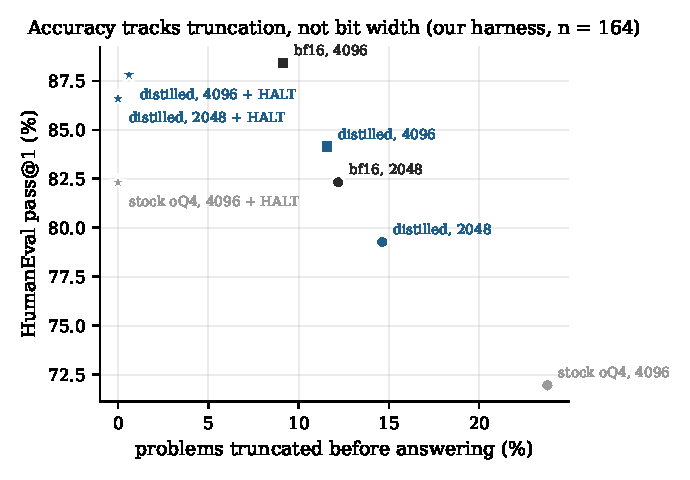
\includegraphics[width=0.8\textwidth]{fig_truncation.pdf}
\caption{The paper in one plot.  Every HumanEval measurement our harness has made on all 164
items, placed by the fraction of problems on which the model never reached an answer.  Bit
width does not order the points; truncation does.  Stars are \HALT{} runs on the same weights
as the circle or square of the same colour.}
\label{fig:truncation}
\end{figure}

\subsection{It is not a scoring artefact}

The natural objection is that a harness which penalises truncation will of
course find truncation explains its scores.  The effect reproduces on a harness
that does not.  oMLX recovers an answer from output ours scores as unfinished,
scoring stock \oQ{} at 87.8\% where ours gives 72.0\%.  On that forgiving
harness the same weights show the effect as \emph{wall clock}: $-33\%$ on
HumanEval, $-15\%$ on MMLU ($+26\%$ on TruthfulQA, where the distilled model
lost).  A model that reaches its answer a third sooner on the benchmark where it
improved, measured by a harness with no truncation penalty at all, is a
property of the model and not of the scoring.

\subsection{The quantization ladder}

\begin{table}[t]
\centering
\caption{The quantization ladder on the same 1{,}000 MMLU questions (oMLX). oQ3 has fewer bits than oQ4 and should be at least as fast per token; it takes 2.23$\times$ as long. bf16's 2.20$\times$ is unquantized compute being slower per token, a different effect. Wall-clock totals, not token counts.}
\label{tab:ladder}
\begin{tabular}{lrrr}
\toprule
Build & MMLU & Seconds & vs oQ4 \\
\midrule
oQ3 & 66.6 & 34,085 & 2.23$\times$ \\
oQ4 & 78.0 & 15,262 & 1.00$\times$ \\
oQ8 & 83.1 & 16,434 & 1.08$\times$ \\
bf16 & 82.6 & 33,507 & 2.20$\times$ \\
\textbf{distilled oQ4} & 83.5 & 13,007 & 0.85$\times$ \\
\bottomrule
\end{tabular}
\end{table}


\begin{figure}[t]
\centering
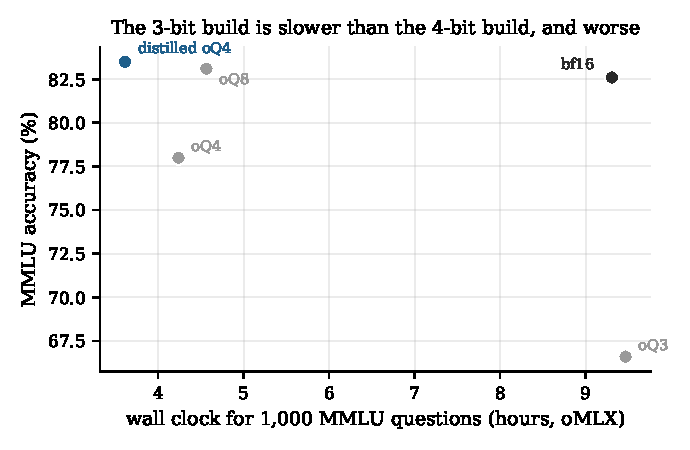
\includegraphics[width=0.7\textwidth]{fig_ladder.pdf}
\caption{The quantization ladder (Table~\ref{tab:ladder}) as accuracy against wall clock for the
same 1{,}000 MMLU questions.  The 3-bit build has fewer bits to multiply than the 4-bit build and
takes 2.2$\times$ as long, because it generates more tokens; the distilled 4-bit build is both the
most accurate and the fastest.}
\label{fig:ladder}
\end{figure}

Table~\ref{tab:ladder} is the strongest single piece of evidence and the one
with the clearest caveat.  The 3-bit build has fewer bits than the 4-bit build,
so its per-token throughput should be at least as high; it takes 2.23$\times$
as long for the same 1{,}000 questions while scoring 11.4 points lower.  The
extra time is extra tokens: it is reasoning at much greater length and arriving
somewhere worse.  These are wall-clock totals, because the external harness
does not emit per-item token counts; the inference is strong but not airtight.

\subsection{Budget sensitivity on unchanged weights}

The bf16 base on our harness, only the budget changed: 82.3\% HumanEval with 20
truncations at 2{,}048 tokens; 88.4\% with 15 at 4{,}096.  Six points of
``model quality'' that are entirely an evaluation parameter---and 15 items
still truncate at the larger budget, so the number never reaches zero, it just
stops mattering as much.

\subsection{Multiple choice hides it}

The repair shows up on code ($+12.2$ on our harness) and barely on multiple
choice (MMLU and TruthfulQA within noise at $n=250$).  That asymmetry is itself
evidence.  A truncated program is worthless; a truncated multiple-choice trace
often still contains a recoverable letter.  \textbf{The benchmark that most
clearly exposes this failure is the one whose output cannot be salvaged.}
Benchmarks that can salvage it will under-report the damage.

\subsection{The teacher does it too}
\label{sec:teacher-termination}

In the on-policy experiment of \S\ref{sec:v8}, the distilled model was rolled
out over a fresh 4{,}974-prompt pool and only its 1{,}247 failures were sent to
the teachers.  The 35B code teacher verified on \textbf{29\%} of those and
\textbf{failed to terminate on 38\%} even after budget escalation to 4{,}608
tokens---against 73\% verified on random prompts from the same pool under the
same teacher and verifier.  On the problems a quantized 9B cannot finish, a
4-bit 35B frequently cannot finish either.  The failure is not specific to the
small model; it is a property of hard problems under a budget, and
quantization moves the threshold.

\section{Repairing it at decode time: \HALT{}}
\label{sec:forcing}

If the failure is stopping, the cheapest test is to stop the model for it.
\HALT{} (Harness-Applied Limit on Thinking) is the closing half of budget
forcing \citep{muennighoff2025s1}: when the reasoning block has not closed by
the time the budget is nearly spent, the harness closes it---appending a
one-line commit phrase and \texttt{</think>}---and allows a reserved number of
tokens for the answer.  Concretely, decoding runs in two phases: $B-N$ tokens, then $N$
more for anything that hit the first cap, with \texttt{</think>} forced only for
items still inside the block.  No item receives more than $B$ tokens in total.
One implementation detail mattered: an earlier version took the reserve out of
\emph{every} item's budget and cut a correct solution mid-answer; the per-item
diff caught it where the aggregate did not.

\begin{table}[t]
\centering
\caption{Budget forcing on the same weights, our harness, reserve $N=256$. \emph{Plain}: standard decoding under the budget. \emph{Forced}: two-phase decoding; items still inside \texttt{<think>} at the phase-1 cap have the block closed for them and receive the reserve to answer. No item receives more than the budget in total.}
\label{tab:forcing}
\resizebox{\textwidth}{!}{%
\begin{tabular}{lllrrrrr}
\toprule
Model & Benchmark & Budget & Plain & Trunc. & Forced & Forced $\to$ correct & $\Delta$ \\
\midrule
v1 & HumanEval & 2{,}048 & 130/164 (79.3) & 24 & 142/164 (\textbf{86.6}) & 12 of 29 & +12 \\
v1 & HumanEval & 4{,}096 & 138/164 (84.2) & 19 & 144/164 (\textbf{87.8}) & 6 of 18 & +6 \\
stock oQ4 & HumanEval & 4{,}096 & \multicolumn{5}{l}{\emph{pending}} \\
v1 & MMLU$_{250}$ & 3{,}072 & \multicolumn{5}{l}{\emph{pending}} \\
\bottomrule
\end{tabular}
}
\end{table}


\begin{figure}[t]
\centering
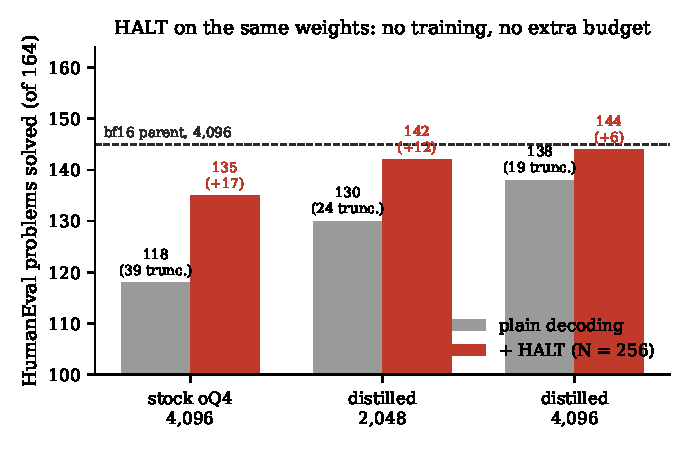
\includegraphics[width=0.75\textwidth]{fig_halt.pdf}
\caption{\HALT{} on the same weights (Tables~\ref{tab:forcing} and \ref{tab:soft}).  Grey: plain
decoding under the budget, with the number of problems truncated before answering.  Red: the hard
form, two-phase decoding with a 256-token reserve.  Blue: the soft form, a \texttt{</think>} logit
ramp from 1{,}024 tokens.  No item receives more total budget in either.  Dashed: the bf16 parent
at 4{,}096 on the same harness.}
\label{fig:halt}
\end{figure}

Table~\ref{tab:forcing} and Figure~\ref{fig:halt} give the result.  On the \textbf{stock} \oQ{}
build---no distillation at all---\HALT{} takes HumanEval from 118 to 135 of 164, \textbf{+10.4
points}, recovering 17 of the 40 items it forced.  Distillation took the same weights from 118 to
138 on this harness; a two-phase decoder alone recovers most of that.  On MMLU, where a truncated
multiple-choice trace is often already salvageable (\S\ref{sec:mechanism}), the effect is
correspondingly smaller: all 10 truncations recovered, 3 of them to a correct answer, +1.2 points.
Two further observations stand out.  First,
\textbf{the distilled model under \HALT{} at 2{,}048 tokens outperforms the
same model allowed 4{,}096 without it}---half the budget, more correct answers.  Forcing is not only
recovering truncations; it is stopping the model before longer reasoning turns
into wrong answers.  Second, in a 24-item pilot, a problem the model reasoned on
to $\approx$2{,}050 tokens and answered \emph{wrong} was answered \emph{right}
when cut at 1{,}792: past some point, continued reasoning has negative value
and the model does not detect it.  Wall clock is unchanged.

\subsection{The soft form: a ramp on the stop logit}
\label{sec:soft}

The hard form places a cliff: reasoning ends at $B-N$ whether or not the model
was one sentence from an answer.  A small series of decode-time probes, each a
30-minute HumanEval run on the same weights, asked what else moves the
truncations.  A repetition penalty of 1.1 does nothing (128 correct, 24
truncated against 130/24 plain) and sampling at $T=0.6$ hurts (122/28); reading
the tail of each truncated trace explains why, since only 2 of 24 loop, while
14 had already written a solution inside the reasoning block and were still
checking it and 8 were reasoning.  Truncation is not degeneration.

The probe that worked is a bias of $s\,(n-n_0)$ added to the \texttt{</think>}
logit at generated position $n>n_0$ while the block is open, and nothing
otherwise.  Before $n_0$ decoding is byte-identical to plain; once the block
closes the processor is inert.  Table~\ref{tab:soft} gives the result at
$n_0=1{,}024$, $s=0.02$.  On the distilled build, 147 of 164, \textbf{+17 over
plain and +5 over the hard form}, with every one of the 130 items plain
decoding solved still solved.  On the \textbf{stock} \oQ{} build, 108 to
\textbf{139}, +18.9 points: 28 of its 48 truncations become correct answers and
3 wrong answers do too, again with no regressions.  For scale, the ramped stock
build at 2{,}048 tokens beats both the hard form on the same build at 4{,}096
(135) and the distilled build decoded plainly at 4{,}096 (138), and the ramped
distilled build beats its own bf16 parent at 4{,}096 (145).  MMLU moves the
same way at its smaller truncation rate: 206 to 210 of 250, no regressions.

\begin{table}[t]
\centering
\caption{Soft \HALT{}: a bias of $0.02\,(n - n_0)$ on the \texttt{</think>} logit while the block is open, for generated position $n > n_0$; nothing before $n_0$, nothing once the block closes. Same weights and budget as \emph{plain}; \emph{hard} is the two-phase limit of Table~\ref{tab:forcing} ($N=256$). \emph{Regr.} counts items correct under plain decoding that the ramp gets wrong.}
\label{tab:soft}
\resizebox{\textwidth}{!}{%
\begin{tabular}{lllrrrrrrrr}
\toprule
 & & & \multicolumn{2}{c}{Plain} & Hard & \multicolumn{4}{c}{Soft ramp} & \\
\cmidrule(lr){4-5} \cmidrule(lr){7-10}
Model & Benchmark & Budget & Correct & Trunc. & Correct & $n_0$ & Correct & Trunc. & Regr. & $\Delta$ vs plain \\
\midrule
v1 & HumanEval & 2{,}048 & 130/164 & 24 & 142 & 1{,}024 & \textbf{147} & 0 & 0 & +17 \\
stock oQ4 & HumanEval & 2{,}048 & 108/164 & 48 & -- & 1{,}024 & \textbf{139} & 0 & 0 & +31 \\
v1 & MMLU$_{250}$ & 3{,}072 & 206/250 & 10 & 209 & 2{,}048 & \textbf{210} & 0 & 0 & +4 \\
v1 & TruthfulQA & 2{,}048 & 583/817 & 67 & -- & 1{,}024 & \textbf{610} & 0 & 0 & +27 \\
\bottomrule
\end{tabular}
}
\end{table}

\begin{table}[t]
\centering
\caption{Ramp sweep on the distilled oQ4 build, HumanEval, 2{,}048-token budget, our harness. The effect is a plateau: any slope from 0.02 and any start from 768 to 1{,}280 closes every block and recovers 14--17 items; 0.01 is too weak to close the block by the budget.}
\label{tab:sweep}
\begin{tabular}{llrrrr}
\toprule
$n_0$ & slope & Correct & Trunc. & Regr. & Mean tokens \\
\midrule
\multicolumn{2}{l}{plain} & 130 & 24 & -- & 1,139 \\
\midrule
1{,}024 & 0.01 & 133 & 17 & 0 & 1,135 \\
1{,}024 & 0.02 & 147 & 0 & 0 & 1,085 \\
1{,}024 & 0.04 & 147 & 0 & 0 & 1,016 \\
768 & 0.02 & 146 & 0 & 1 & 1,032 \\
1{,}280 & 0.02 & 144 & 0 & 0 & 1,126 \\
\bottomrule
\end{tabular}
\end{table}


Table~\ref{tab:sweep} shows the setting is not delicate.  Any slope from 0.02
and any $n_0$ from 768 to 1{,}280 closes every block by the budget and lands
between 144 and 147; only $s=0.01$ is too weak to matter.  Mean output length
falls with the ramp (1{,}139 to 1{,}085 tokens at $s=0.02$), so it is also
cheaper.  The five items that go from wrong to right are ones that reasoned
past 1{,}024 tokens to a wrong answer under plain decoding and answer
correctly when stopping is made cheaper: the pilot observation above, at
$n=5$.

\paragraph{It is not a quantization repair.}
The natural control is the full-precision parent.  Table~\ref{tab:generality}
and Figure~\ref{fig:generality} run the same ramp on every build of the
quantization ladder and on the 35B teacher.  \textbf{bf16 gains +17}, exactly
what the distilled 4-bit build gains, and bf16 ramped at 2{,}048 tokens (152)
beats bf16 decoded plainly at 4{,}096 (145).  The 35B teacher, already at 151,
gains +8 and truncates nothing.  On every build from 4 bits up the ramp recovers
two thirds to four fifths of whatever truncated; at 3 bits it recovers 41\%,
because more of what the 3-bit model fails to finish it also cannot solve.
One item regressed in 735 previously-correct items across the six builds.

\begin{table}[t]
\centering
\caption{The soft ramp across the quantization ladder, the 35B teacher, and two other architectures, HumanEval, 2{,}048-token budget, our harness, $n_0 = 1{,}024$, $s = 0.02$. The gain tracks the truncation count on every build, full precision included; \emph{Regr.} is items correct under plain decoding that the ramp gets wrong.}
\label{tab:generality}
\begin{tabular}{lrrrrrrr}
\toprule
 & \multicolumn{2}{c}{Plain} & \multicolumn{2}{c}{Ramp} & & & \\
\cmidrule(lr){2-3} \cmidrule(lr){4-5}
Build & Correct & Trunc. & Correct & Trunc. & $\Delta$ & Regr. & $\Delta$ / Trunc. \\
\midrule
oQ3 & 75 & 78 & \textbf{107} & 1 & +32 & 1 & 0.41 \\
oQ4 (stock) & 108 & 48 & \textbf{139} & 0 & +31 & 0 & 0.65 \\
oQ4 (distilled, v1) & 130 & 24 & \textbf{147} & 0 & +17 & 0 & 0.71 \\
oQ8 & 136 & 26 & \textbf{154} & 0 & +18 & 0 & 0.69 \\
bf16 parent & 135 & 20 & \textbf{152} & 0 & +17 & 0 & 0.85 \\
Ornith-1.5-35B-A3B 4-bit (teacher) & 151 & 10 & \textbf{159} & 0 & +8 & 0 & 0.80 \\
\midrule
Qwen3.8-27B 4-bit (dense) & 116 & 44 & \textbf{147} & 0 & +31 & 0 & 0.70 \\
Qwen3.6-35B-A3B 4-bit (MoE) & 27 & 135 & \textbf{147} & 0 & +120 & 0 & 0.89 \\
\bottomrule
\end{tabular}
\end{table}


\begin{figure}[t]
\centering
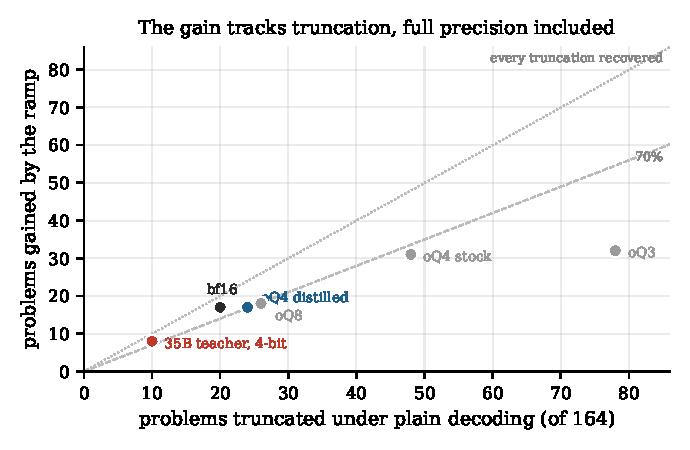
\includegraphics[width=0.62\textwidth]{fig_generality.pdf}
\caption{Ramp gain against plain-decoding truncation count, one point per build,
HumanEval at 2{,}048 (Table~\ref{tab:generality}).  The dotted line is every
truncation recovered; the dashed line is 70\%.  Full precision sits on the same
line as the quantized builds.}
\label{fig:generality}
\end{figure}

So the reading has to be narrower than ``quantization broke stopping and the
ramp repairs it.''  Every reasoning build here, the full-precision one
included, runs past the point where more reasoning helps when decoded greedily
under a finite budget, and a position-dependent bias on the stop token repairs
that in all of them.  What quantization does is raise how often it happens
(20, 26, 48 and 78 truncations from bf16 down to 3 bits), so the quantized
builds have the most to recover; that is why the diagnosis in
\S\ref{sec:mechanism} found termination dominating the measured quantization
damage.  The hard form was the coarse version of the same repair.  Two attempts
to move it into the weights are reported in \S\ref{sec:v9v10}; both failed,
which is consistent with the behaviour living in the decoding procedure rather
than in anything the training data can teach.

\HALT{} generalises to any model with this failure mode, including the stock
build we would have shipped without distillation, and it needed no training.
The soft form is the one we recommend: one logits processor, no phase
boundary, and a worst case identical to plain decoding.

\section{What did not work, and what the controls established}
\label{sec:negative}

\begin{table}[t]
\centering
\caption{Every training run after v1, each moving one variable, each with a prediction recorded before measurement. oMLX, same protocol as Table~\ref{tab:main}. v5 was abandoned after MMLU (5.4$\times$ v1's wall clock). Across the six completed comparable runs, 21 of 24 deltas are negative and none is positive beyond noise.}
\label{tab:runs}
\resizebox{\textwidth}{!}{%
\begin{tabular}{llrrrl}
\toprule
Run & Change from v1 & MMLU & TruthfulQA & HumanEval & $\Delta$ vs v1 \\
\midrule
\textbf{v1} & baseline recipe & 83.5 & 79.0 & 90.8 & --- \\
\midrule
v2 & misconception slice replaces TriviaQA; brief code & 83.1 & 76.9 & 85.4 & -0.4 / -2.1 / -5.4 \\
v3 & abstention slice added; v1 code traces restored & 83.6 & 77.4 & 87.2 & +0.1 / -1.6 / -3.6 \\
v4 & 1{,}024-token length bias removed, all else held & 83.2 & 76.6 & 89.6 & -0.3 / -2.4 / -1.2 \\
v5 & objective $\to$ 0.3\,CE + 0.7\,KL(teacher$\|$student), top-64 & 77.2 & -- & -- & -6.3 / -- / -- \\
v7 & adapter rank 32 $\to$ 64, data byte-identical & 83.2 & 77.6 & 88.4 & -0.3 / -1.4 / -2.4 \\
v8 & on-policy: v1's own failures, continued from v1 & 81.6 & 76.3 & 85.4 & -1.9 / -2.7 / -5.4 \\
v8-ctl & same recipe, random prompts (control) & 83.2 & 77.7 & 86.6 & -0.3 / -1.3 / -4.2 \\
v6 & filter $\to$ recover verified abstentions & \multicolumn{4}{l}{stopped before training: 22 usable traces, 0 under the cap} \\
\bottomrule
\end{tabular}
}
\end{table}


\begin{figure}[t]
\centering
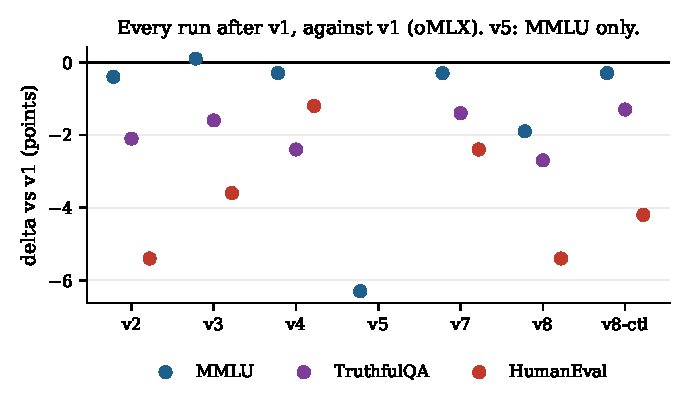
\includegraphics[width=0.75\textwidth]{fig_runs.pdf}
\caption{Every completed run after v1, as its delta against v1 on each benchmark (oMLX).
Twenty-one of twenty-four deltas are below zero and none is above it beyond noise.  v5 was
abandoned after MMLU.}
\label{fig:runs}
\end{figure}

Table~\ref{tab:runs} and Figure~\ref{fig:runs} list every run after v1.  Each moved one variable, each
had a prediction recorded before measurement, and each was measured on oMLX
under the protocol of Table~\ref{tab:main}.  Across the six completed
comparable runs, \textbf{21 of 24 benchmark deltas against v1 are negative and
none is positive beyond noise}.  v1 is not merely the best result; it behaves
like a sharp optimum that every perturbation moves away from.

\subsection{Data composition (v2--v4)}

MMLU sat at 83.5, 83.1, 83.6, 83.2 across mixtures differing in source, volume
(1{,}672 to 4{,}075 samples) and length distribution, and v1 already matches its
35B teacher there.  v4 is the cleanest: v1 had trained only on traces under
1{,}024 tokens---1{,}758 of median 678, while 1{,}735 of median 1{,}449 were
never seen---which \S\ref{sec:mechanism} predicts should matter.  Lifting the cap
to 2{,}048 with sample count, steps and every hyperparameter held, and a
\texttt{max\_samples} cap added so the length change could not smuggle in
volume, moved nothing.  The pre-registered prediction (HumanEval improves most)
was wrong.  Telling the code teacher to be brief in v2 cost 5.4 points of
HumanEval; asking for shorter abstention traces in v3 produced \emph{longer}
ones.  Brevity instructions do not reliably work on these models.

\subsection{Objective: forward KL makes the model unable to stop (v5)}
\label{sec:v5}

v5 trained against the teacher's renormalised top-64 next-token distribution
(measured to hold 99.93\% of its mass) with loss
$0.3\,\mathrm{CE} + 0.7\,\mathrm{KL}(p_T \,\|\, p_S)$, everything else at v1.  It
produced the first model \emph{below stock}: 77.2 MMLU in \textbf{69{,}897
seconds against v1's 13{,}007} on the same questions---5.4$\times$.  It did not
become confused; it became unable to stop.  This is the mode-covering failure
\citet{gu2023minillm} describe: a 9B at 4.7 bits cannot cover a 35B's
low-probability modes, and one of those modes is the teacher's residual
uncertainty about whether to continue reasoning.  Three failure modes were ruled
out before accepting the result (vocabulary identity across teachers, top-$k$
coverage, span alignment) and a latent batcher bug was found and fixed on the
way.  v7 later confirmed the collapse is specific to the objective: a different
departure from v1 left wall clock normal.

\subsection{Adapter capacity (v7)}

Every earlier run used rank 32 over the top 16 layers, chosen once and never
revisited.  Doubling to 86.6M trainable parameters on byte-identical data
(sha256-verified) changed nothing: all three deltas inside one standard error,
wall clock normal.  Rank 64 across all 32 layers does not fit in 64\,GB---backprop
\emph{depth}, not rank, is what costs.  This converts ``capacity, not recipe''
from an inference reached by eliminating recipes into a measurement.

\subsection{The TruthfulQA regression is an abstention deficit the teacher cannot fix (v3, v6)}
\label{sec:truthfulqa}

Per item, v1 matches stock on ordinary TruthfulQA questions (81.3\% vs 81.4\%)
and \textbf{loses 11 points on the 117 whose correct answer expresses
uncertainty} (65.0\% vs 76.1\%; 19 lost, 6 gained, $p\approx0.016$).  Rejection
sampling keeps only confident correct answers, so the student never sees
warranted uncertainty.  Adding 527 SQuAD-v2 unanswerable items (v3) moved
TruthfulQA \emph{down} 1.6: reading-comprehension abstention is a different
skill.  Changing the filter instead (v6)---re-asking the teacher, with its
confidence made explicit, the 122 open-ended prompts it had answered wrong, and
keeping only the traces where it declined---yielded 22 usable traces, of which
none fit the training cap.  The number that matters is the other one:
\textbf{on questions it had already answered wrong, invited to say it did not
know, Qwen3.6-35B re-asserted a confident answer 82\% of the time.}
Sequence-level distillation can only transmit what the teacher emits, and this
teacher does not emit calibrated uncertainty.  v6 was stopped before training
on a threshold set in advance.

\subsection{A second training pass from the best checkpoint is itself harmful (v8 and its control)}
\label{sec:v8}

v8 tested on-policy prompt selection in the spirit of \citet{agarwal2023gkd} at
the prompt level: roll v1 out over a fresh pool of 4{,}974 prompts (a different
seed, every v1 prompt excluded, code from KodCode since MBPP was exhausted), keep
the 1{,}247 it fails, have the teacher answer only those, train on the 330 that
verify, continuing from v1's fused checkpoint.  A control arm trained on 330
\emph{random} prompts from the same pool with everything else identical.
\textbf{Both arms lost to v1 on all three benchmarks by similar amounts}
(Table~\ref{tab:runs}).  Since the arms differ only in prompts, the second pass
is the damage, not the selection.  Every method that starts from v1 must first
beat a 1--4 point tax; every method that starts from the base must re-earn v1's
gains.  Three bugs surfaced during this run and are fixed in the released
code: a verifier ordering that scored model-copied test calls as
\texttt{NameError}s, a batching loop that silently dropped prompts at every
domain boundary (present since v1), and rollouts that did not store answer text.

\subsection{The \HALT{} behaviour does not train into the weights (v9, v10)}
\label{sec:v9v10}

If a decode-time bias repairs stopping, can the repair be distilled into the
weights so no harness is needed?  Two attempts, each with a go/no-go set before
the run.  \textbf{v9} rolled the distilled build out under the hard form over
the 4{,}974-prompt pool and kept every verified-correct trace, tagging those
the harness had closed, to train on.  The yield was the problem: at a
1{,}536-token budget the model solved 21\% of the pool's code and only 27 of
911 forced traces verified; at 2{,}304 it solved 34\% and 7 of 551 forced
traces verified.  The pool is harder than HumanEval, and an item still reasoning
at the budget there has usually not reached an answer to commit to.  Below the
150-trace threshold, nothing was trained.  \textbf{v10} used the abundant
negative instead: 378 pairs of a verified teacher trace against the student's
own unterminated trace on the same prompt, trained with sigmoid DPO
\citep{rafailov2023dpo} plus a cross-entropy term on the chosen trace, reference
fixed at v1, factorised into three single-sequence passes so a 3{,}072-token
pair fits in 35\,GB.  The loss reached zero within 50 steps (the pairs are
trivially separable) and the margin kept growing; at both the final and an
early checkpoint the model truncated \emph{more} than v1 (30 and 39 against
24) and lost 7--14 items, with gains and losses symmetric across problems.
Sequence-level preference moves the likelihood of whole traces; stopping is a
decision at one token, and nothing in the pair localises credit there.  A
feasibility check for verifier-reward RL found that 59\% of prompt groups in
the pool had no correct sample among eight, so that route was not taken.

\section{Engineering: a chunkwise training path for gated DeltaNet}
\label{sec:engineering}

Training was pinned at 1{,}024-token sequences, which rejected 46\% of every
trace generated---six times what wrong answers cost.  The cause was not the
hardware.  \texttt{mlx\_lm} \citep{mlx2023} trains GDN layers through a
sequential Python loop over every timestep, because the fast Metal kernel used
at inference has no gradient; its own docstring calls it a reference
implementation for prefill.  Measured: $\approx$8\,MB of autograd state per
token per layer.

The gated delta rule admits a chunkwise-parallel form
\citep{yang2024deltanet,yang2024gated} that keeps $O(T/C)$ materialised states
instead of $O(T)$.  Two details mattered in MLX.  \texttt{mx.linalg.tri\_inv}
is CPU-only with no VJP, so the unit-triangular inverse is built from matmuls by
$2\times2$ block recursion in $\log_2 C$ levels, which autodiff handles
natively.  And the textbook derivation divides by the cumulative decay, which
underflows on strongly decaying heads and sends intermediate writes to
infinity; carrying bounded ratios $G_j/G_i \le 1$ instead is what makes it work
on a real model.  A fused Metal triangular \emph{solve} with a hand-written VJP
then replaces the inverse, which was used exactly once as $A^{-1}b$ and cost
5.07 of the 9.3\,ms per chunk.

One GDN layer, forward and backward, cumulative against stock \texttt{mlx\_lm}
at 4{,}096 tokens: \textbf{108.33\,GB / 39.02\,s $\to$ 4.60\,GB / 0.29\,s---24$\times$
memory, 135$\times$ speed}.  Outputs match the sequential reference to
$\sim$$3\times10^{-7}$ relative in fp32 across all five gradients; the inference
kernel matches at 100\% top-1 on the full 9B.  End-to-end training throughput
doubled (55$\to$111 tokens/s) and 2{,}048-token training fits in 41.8\,GB.
Contributed as \PRURL{} (chunkwise path, five model families), with the fused
solve queued behind it.

\section{Related work}

\paragraph{Distillation objectives.}
\citet{hinton2015distilling} and \citet{kim2016sequence} define logit-level and
sequence-level distillation respectively; v1 is the latter with a verifier in
the loop.  \citet{gu2023minillm} argue forward KL is mode-covering and ill-suited
to generative distillation; \citet{agarwal2023gkd} add on-policy sampling and
generalised divergences; \citet{ko2024distillm} propose skew KL;
\citet{shing2025taid} interpolate the target toward the teacher over training.
Our v5 is a direct instance of the forward-KL failure these predict, with
termination as the specific casualty.

\paragraph{Test-time compute.}
\citet{muennighoff2025s1} introduce budget forcing to \emph{extend} reasoning
with ``Wait''; we use the closing half of the same mechanism on a quantized
model and find that forcing \emph{earlier} than the model would stop itself
improves accuracy.

\paragraph{Quantization-aware training and rotation.}
EfficientQAT \citep{chen2024efficientqat} and Recover-LoRA
\citep{recoverlora2025} train through the quantizer; QuaRot
\citep{ashkboos2024quarot} suppresses outliers before it.  We trained in bf16
and quantized last, and \S\ref{sec:v8}'s finding that continued training from
the best checkpoint is harmful bears on whether a second, quantization-aware
pass could help here.

\paragraph{Linear attention.}
\citet{yang2024deltanet,yang2024gated} give the chunkwise delta-rule form
\S\ref{sec:engineering} implements.  \citet{wijmans2024cce} remove the logit
memory that a 248k vocabulary costs and would compound with logit-level
distillation.  \citet{marathe2026bytes} distil token-level teachers into
byte-level students for pretraining; their objective is forward KL, and their
setting---a student with no prior distribution to disturb---is one where the
failure in \S\ref{sec:v5} does not arise.

\section{Threats to validity}

\paragraph{Scope.}
One model family, one quantization scheme, one hardware target; the ramp was
measured on two model sizes and five bit widths of that family.  The
\emph{mechanism} behind the quantized model's verbosity is documented, not
explained: we show that a coarser weight grid produces longer reasoning and that
this dominates the measured damage, not why.  The ramp's effect on the
full-precision parent (\S\ref{sec:soft}) means the repair addresses a property
of greedy budgeted decoding that quantization amplifies, not one it creates;
we have not tested whether other model families amplify it the same way.

\paragraph{Measurement.}
The quantization-ladder timing (\S\ref{sec:mechanism}) is wall clock, not
token counts, because the external harness does not emit them.  The two
harnesses disagree by 15 points on the stock model's absolute HumanEval while
agreeing on every direction; any single absolute number should be read as
approximate.  MMLU is a 1{,}000-question sample; TruthfulQA and HumanEval are
complete.  Standard errors for the run comparisons are single-proportion
bounds (paired errors are tighter), so the ``inside noise'' claims are
conservative.

\paragraph{Unexplained results.}
In the v8 experiment the random-arm model became 46--80\% slower to answer
while the failure-arm model barely changed.  The failure arm's traces are by
selection the ones a 35B finished cleanly, which may be the one thing
error-conditioning did; server load during the control run cannot be
excluded.  Recorded, not claimed.

\paragraph{What was not run.}
Token-level on-policy distillation with a mode-seeking divergence and
termination-token masking; quantization-aware self-distillation from the bf16
distilled model into its own \oQ{} build; full-parameter updates via a factored
optimiser.  \S\ref{sec:v8} constrains all three.  TruthfulQA has no verifier and
its regression was not repaired.

\section{Conclusion}

A reasoning model decoded under a budget runs past the point where reasoning
helps, and a 4-bit one does so most: its dominant failure is that it does not
stop.  We found
this the slow way: one distillation run that worked, nine that did not, and a
control that showed trying harder from the best checkpoint makes it worse.
Reading the per-item records and the timing column is what turned the negative
results into a diagnosis, and the diagnosis into two interventions that needed
no training, of which the softer one---make stopping gradually cheaper and let
the model choose---is the better and the simpler, and works on the
full-precision model too.  The practical recommendations are short.  Report
truncation rates next to accuracy.  Measure generation length before and after
quantizing; wall clock is the cheapest early warning.  And treat the token
budget as part of the model being evaluated, because for a reasoning model it
is.

\section*{Reproducibility}

Code, configurations, every run's adapters, fused checkpoints, teacher traces,
per-item evaluation records and a 53-section decision log are at \RepoURL{}.
\texttt{benchmarks/baseline.json} holds every number in this paper with its
measurement date and harness; \texttt{scripts/make\_paper\_tables.py}
regenerates every table in this paper from those files.
\texttt{odistil eval --force-budget N} reproduces the hard form of \HALT{} and
\texttt{--think-bias 1024:0.02} the soft form (\S\ref{sec:forcing}).

\bibliography{references}
\bibliographystyle{plainnat}

\end{document}
